\documentclass[tikz,border=3.14mm]{standalone}
\usepackage{pgfplots}
\pgfplotsset{compat=1.16}
\begin{document}
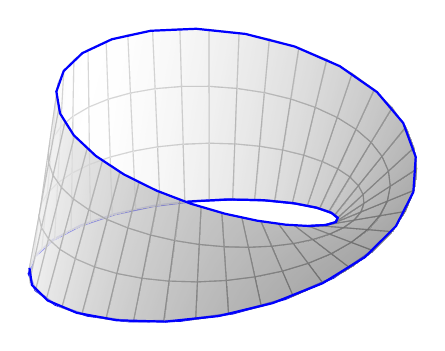
\begin{tikzpicture}
   \begin{axis}[
         hide axis,
         view = {40}{40}
      ]
      \addplot3 [color=blue,thick,
         domain     = 360:720,samples y=0,
      ] (
      {(1+0.5*0.5*cos(x/2)))*cos(x)},
      {(1+0.5*0.5*cos(x/2)))*sin(x)},
      {0.5*0.5*sin(x/2)}
      );
      \addplot3 [
         surf,
         colormap={blackwhite}{gray(0cm)=(1); gray(1cm)=(0.5)},
         shader     = faceted interp,opacity = 0.7,
         %shader = interp,
         point meta = x,
         samples    = 40,
         samples y  = 4,
         z buffer   = sort,
         domain     = 0:360,
         y domain   =-0.5:0.5
      ] (
      {(1+0.5*y*cos(x/2)))*cos(x)},
      {(1+0.5*y*cos(x/2)))*sin(x)},
      {0.5*y*sin(x/2)}
      );
      \addplot3 [color=blue,thick,
         domain     = -140:497.5,samples y=0,samples=(640/360)*24+1,
      ] (
      {(1+0.5*0.5*cos(x/2)))*cos(x)},
      {(1+0.5*0.5*cos(x/2)))*sin(x)},
      {0.5*0.5*sin(x/2)}
      );
   \end{axis}
\end{tikzpicture}
\end{document}